\vspace{\parskip}
Today we will use {\scshape Desmos} 
to explore the effects of $\bm{a}$, $\bm{h}$, $\bm{k}$ 
on \gap{transformed} absolute value functions. 

\begin{tcolorbox}[center,width=2.5in,valign=center,]
    \large
    \vspace{-\baselineskip}
    \[ f(x) = \bm{a}\,|x-\bm{h}|+\bm{k} \]
\end{tcolorbox}

\vfill 

\begin{myAnnotate}{{Activity}}{To join the {Desmos} activity\dots}[%
    center,
    width=5.5in,
    before skip = 1\baselineskip,
    colbacktitle=black!15,
    ]
    \begin{itemize}[nosep]
        \item Get out your phone.
        \item Open a browser to {\bfseries\ttfamily student.desmos.com}.
            \begin{center}
                \fbox{
\includegraphics[width=3in]{../student-desmos-com}}
            \end{center}
        \item Join with this code: {\bfseries\ttfamily USHJMS}.
        \item Do \myEmph{not} login.
        \item A \myEmph{small screen} is OK.
        \item There are 4 screens in the activity. 
            \begin{center}
                \fbox{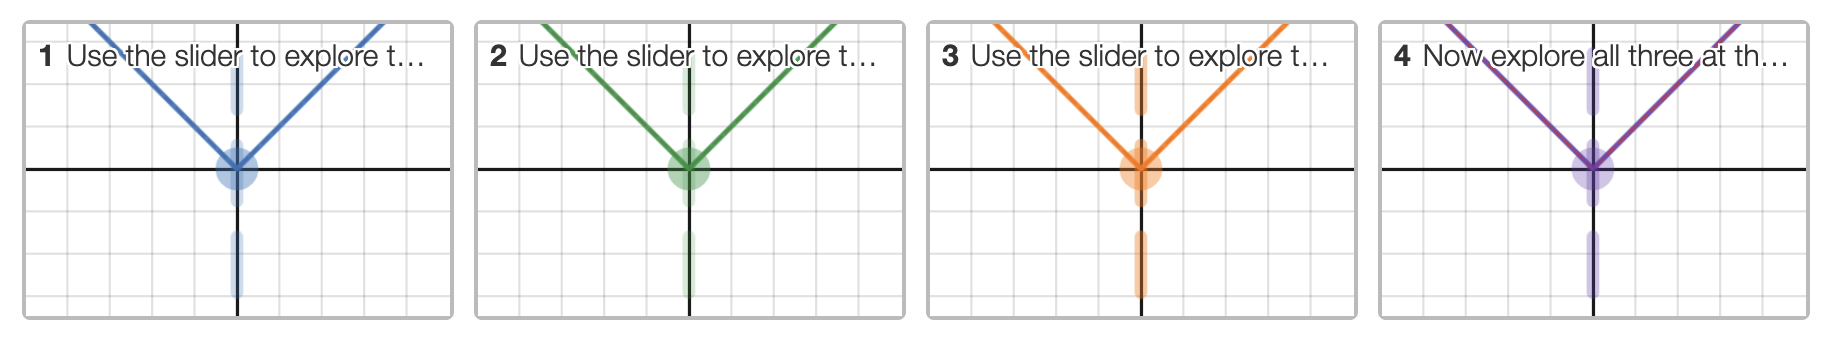
\includegraphics[width=4in]{../4-desmos-screens.png}}
            \end{center}
        \item Go through them one at a time.
        \item Answer the questions on the worksheet.
    \end{itemize}
\end{myAnnotate}

\vfill{}